\documentclass[11pt]{article}

\usepackage[T1]{fontenc}
\usepackage{newtxtext}
\usepackage{newtxmath}
\usepackage{microtype}
\usepackage{amsmath}
\usepackage[margin=1in]{geometry}
\usepackage{booktabs}
\usepackage{caption}
\usepackage{subcaption}
\usepackage[hidelinks]{hyperref}
\usepackage{float}
\usepackage{placeins}
\usepackage{needspace}
\usepackage{indentfirst}
\usepackage{enumitem}
\usepackage{titlesec}
\usepackage{tikz}
\usepackage{pgfplots}
\pgfplotsset{compat=1.18}
\usetikzlibrary{positioning,arrows.meta,shapes.geometric,fit}
\usepackage[numbers,sort&compress]{natbib}

\setlength{\parindent}{1.25em}
\setlength{\parskip}{0pt}
\captionsetup{font=small, labelfont=bf, skip=4pt}

\titleformat{\section}{\normalfont\large\bfseries}{\thesection}{0.5em}{}
\titleformat{\subsection}{\normalfont\normalsize\bfseries}{\thesubsection}{0.5em}{}
\titleformat{\subsubsection}{\normalfont\normalsize\bfseries}{\thesubsubsection}{0.5em}{}
\titlespacing*{\section}{0pt}{0.9em}{0.45em}
\titlespacing*{\subsection}{0pt}{0.65em}{0.3em}
\titlespacing*{\subsubsection}{0pt}{0.5em}{0.2em}

\newcommand{\code}[1]{\texttt{#1}}
\newcommand{\aegis}{Aegis}
\newcommand{\mcpshield}{MCPShield}
\newcommand{\seagent}{SEAgent}
\newcommand{\agentguardian}{AgentGuardian}

\title{MCP Gateway: Secure Federated Access to Enterprise Tool Servers}

\author{Harish Gaggar\\
  Intuit Inc., Mountain View, CA, USA\\
  \texttt{harish\_gaggar@intuit.com}}

\date{}

\begin{document}
\maketitle

\begin{abstract}
\noindent
The Model Context Protocol (MCP) enables agents to call tools on remote servers, but it does not specify how enterprises expose many backends through one auditable entry point, enforce tenant isolation on tool names, or keep upstream credentials off the agent host.
We define that missing \emph{control plane} as an MCP Gateway: a single URL where every request is authenticated, rate-limited, authorized on MCP methods and tool resources, then routed or answered from a federated catalog.
The paper gives reusable material others can adopt: a reference OAuth/JWE architecture, a cross-method attribute-based access control (ABAC) model, a documented threat model, and an open research implementation with benchmarks.
On a public testbed, 13/13 automated tests pass; median \code{tools/call} overhead is 0.43\,ms; peak throughput is 3{,}699 requests per second; policy evaluation scales linearly to 72.9\,$\mu$s at 200 rules; and a GAP-style harness shows forbidden cross-tenant calls blocked at the gateway (HTTP 403) but not on a direct path.
Evaluation is limited to loopback measurements without live frontier models; the artifact documents extension protocols for TLS, WAN, and agent-level studies.
\end{abstract}

\section{Introduction}
\label{sec:intro}

MCP~\cite{anthropic2024mcp} standardizes how agents discover and invoke tools on remote servers using JSON-RPC over HTTP.
Common methods include \code{tools/list} (what tools exist?) and \code{tools/call} (run a named tool with parameters).
Enterprises are standing up many MCP servers at once: filesystem access, databases, ticketing, source control, and more.
Each server usually has its own URL, OAuth registration, and tool catalog.

\textbf{A running example.}
Suppose two internal teams share one agent platform.
Team~A should use filesystem tools only; Team~B should use database tools only.
Without a gateway, the agent must store two base URLs, two OAuth tokens, and two catalogs.
A mistaken or malicious \code{tools/call} can hit the wrong backend, and auditors must correlate logs across services by hand.
Section~\ref{sec:problem} formalizes this situation; Sections~\ref{sec:design}--\ref{sec:eval} show how one gateway URL, qualified tool names (\code{fs:read\_file} vs.\ \code{db:query}), and deny-override policy address it.

\textbf{How to read this paper.}
Section~\ref{sec:problem} states the gaps and goal.
Section~\ref{sec:related} positions the gateway next to MCP itself, HTTP gateways, and agent-security research.
Section~\ref{sec:design} is the technical core (request pipeline, policy, routing, threats).
Section~\ref{sec:engineering} maps the design to a deployable OAuth/JWE stack and to our open prototype.
Section~\ref{sec:eval} reports what we measured on that prototype and what we did not.
Section~\ref{sec:discussion} answers common design questions and lists limits.

\subsection{Problem statement}
\label{sec:problem}

We formulate the control-plane problem for multi-tenant enterprise agent deployments.

\textbf{Setting.}
Let $\mathcal{S}=\{s_1,\ldots,s_n\}$ be MCP servers, each exposing a set of tools.
Let $\mathcal{P}$ be principals (teams, services, or users) that run agents.
Every call should satisfy policy: principal $p$ may only use tools and MCP methods allowed for $p$.
When possible, agents should not hold long-lived upstream OAuth tokens for every backend; the platform should broker credentials.

\textbf{What goes wrong without a gateway.}
In the running example, Team~A's agent might still reach \code{db:query} if it knows the database server's URL, even when the model's chat reply says ``I cannot do that.''
Security then depends on model behavior instead of infrastructure.
Operators also lack a single place to attach rate limits, audit logs, and consistent deny rules across \code{tools/call}, \code{tools/list}, \code{resources/read}, and \code{prompts/get}.

\textbf{Three gaps in today's practice.}
\begin{enumerate}[leftmargin=*, itemsep=0.25em]
  \item \textbf{No federation layer.} MCP does not say how to present one merged \code{tools/list} across servers or how to route \code{tools/call} with stable qualified names (\code{namespace:tool}).
  \item \textbf{No method-aware authorization.} Classic HTTP API gateways authorize URLs and TLS identities. They do not treat the MCP method plus tool or resource name as one policy decision.
  \item \textbf{Weak infrastructure safety.} Textual refusal in the model does not guarantee the tool call is blocked on the wire (the GAP phenomenon~\cite{gap2026}). Enforcement must happen on the path the runtime actually uses.
\end{enumerate}

\textbf{Goal.}
Provide one gateway endpoint that (i)~authenticates the agent, (ii)~evaluates policy before any upstream call, (iii)~routes to the correct server or returns a federated catalog, and (iv)~supports observability and credential patterns that other teams can reproduce from this paper and artifact.

\subsection{Solution outline}
\label{sec:solution}

We address the problem in Section~\ref{sec:problem} with one \emph{MCP Gateway}: a single URL that sits between agents and many MCP backends.
Agents never talk to each backend directly; every JSON-RPC request follows the same pipeline in Figure~\ref{fig:flow}.
First the gateway identifies the caller, then applies rate limits, then runs policy \emph{before} any upstream contact.
If the call is allowed, routing selects the backend (using qualified names such as \code{namespace:tool}); for discovery, the gateway can return one merged \code{tools/list} instead of many separate catalogs.
Table~\ref{tab:policy-map} and Equation~\eqref{eq:policy} show how each MCP method maps to a policy resource $\rho(r)$, so authorization applies to \code{tools/call}, \code{tools/list}, \code{resources/read}, and \code{prompts/get} in one place rather than only to HTTP paths.

The paper connects that idea to material others can reuse in four steps, from design to evidence:
\begin{enumerate}[leftmargin=*, itemsep=0.25em]
  \item \textbf{Reference architecture} (Section~\ref{sec:ref-arch}) documents how operators usually implement the gateway: OAuth at the edge, short-lived JWE credentials for agents (upstream tokens stay at the gateway), namespace proxying to backends, Redis-backed session state, and OpenTelemetry-friendly tracing for audits.
  \item \textbf{Policy and threat model} (Sections~\ref{sec:policy}, \ref{sec:threat}) turns the pipeline into concrete rules and risks: deny-override attribute-based access control (ABAC), a threat table aligned with \mcpshield~\cite{mcpshieldFormal2026}, and Table~\ref{tab:compare}, which shows how argument-level systems (\aegis, Progent) and workflow controls (\seagent) complement rather than replace the outer gateway.
  \item \textbf{Open prototype} (repository \code{mcp-gateway-research}) implements the same lifecycle on a federated \code{/gateway/mcp} endpoint with YAML policy and a cached catalog, so readers can run the design rather than infer it from diagrams alone.
  \item \textbf{Evaluation kit} (Section~\ref{sec:eval}) attaches tests and scripts to that prototype: correctness suites, latency and throughput microbenchmarks, a GAP-style cross-tenant harness, and Table~\ref{tab:scope}, which separates what we measured on loopback from planned TLS, WAN, and live-agent extensions.
\end{enumerate}

In short, the gateway is the \emph{outer} enforcement point on the network path.
A standard HTTP reverse proxy is not enough for MCP because it does not merge tool catalogs or authorize JSON-RPC methods and tool names.
Deeper checks on tool arguments or multi-step plans belong inside or behind this layer; they add defense in depth but still assume one auditable front door.

\section{Related Work}
\label{sec:related}

Prior work touches model capability, transport, or inner-loop safety.
This paper focuses on the \emph{missing middle}: operator-facing control in front of many MCP servers.
Table~\ref{tab:compare} summarizes how the gateway relates to the closest systems; the subsections below group the literature by concern.

\subsection{Tool and agent benchmarks}

ToolLLM~\cite{qin2023toolllm}, Gorilla~\cite{patil2023gorilla}, and API-Bank~\cite{li2023apibank} ask whether a model picks the right tool for a task.
They do not provide a deny-override policy engine, federated catalogs, or credential brokering for enterprise fleets.
Benchmarks inform agent quality; they do not replace the gateway gaps in Section~\ref{sec:problem}.

\subsection{API and MCP infrastructure}

REST gateways~\cite{richardson2007rest} and Envoy~\cite{howard2019envoy} terminate TLS, route HTTP paths, and apply coarse auth.
They were not designed to merge MCP \code{tools/list} results or to authorize \code{namespace:tool} inside a JSON-RPC body.
MCP~\cite{anthropic2024mcp} defines the protocol between client and server; it intentionally stops short of multi-tenant federation and org-wide policy.
Our contribution is architectural material for that layer, not a change to the MCP spec.

\subsection{Security and governance for agents}

Agent-security research often targets \emph{what} is said or \emph{what} is in tool arguments.
The gateway targets \emph{whether the call may reach a backend at all}, on the shared URL agents already use.

Table~\ref{tab:compare} summarizes positioning.
\aegis~\cite{aegis2026} and Progent~\cite{progent2025} inspect tool arguments before execution.
GAP~\cite{gap2026} separates textual refusal from tool-call safety; our harness measures the infrastructure slice of that gap.
\mcpshield~\cite{mcpshieldFormal2026} provides threat taxonomies and attestation-oriented controls; we adopt its trust-boundary vocabulary in Section~\ref{sec:threat}.
\seagent~\cite{seagent2026} applies MAC to multi-step workflows; the gateway does not track call graphs but can host a workflow PDP hook.
Policy-first tooling~\cite{policyFirstTooling2025} and \agentguardian-style workflow guards~\cite{agentGuardian2025} enforce plans and approvals inside the agent loop; the gateway remains the outer policy enforcement point (PEP) for MCP transport.

\begin{table}[H]
\centering
\caption{Complementary MCP security layers.}
\label{tab:defenses}
\small
\begin{tabular}{@{}lcccc@{}}
\toprule
Capability & Gateway & \aegis{} / Progent & \mcpshield & \seagent \\
\midrule
Single entry URL & Yes & No & Partial & No \\
Federated \code{tools/list} & Yes & No & Partial & No \\
Tenant / tool ABAC & Yes & Partial & Yes & Partial \\
Argument checks & No & Yes & Partial & No \\
Workflow MAC & No & No & Partial & Yes \\
\bottomrule
\end{tabular}
\end{table}

\begin{table}[H]
\centering
\caption{Comparison to closely related agent-security systems.}
\label{tab:compare}
\footnotesize
\begin{tabular}{@{}lccccc@{}}
\toprule
Work & Entry control & Tool ABAC & Args & Workflow & Formal model \\
\midrule
MCP Gateway (this paper) & Yes & Yes & No & Hook & Threat table \\
\aegis{} / Progent & Partial & No & Yes & No & No \\
\mcpshield & Partial & Partial & Partial & Partial & Yes \\
\seagent & No & Partial & No & Yes & MAC \\
GAP (metric) & No & No & No & No & TC vs.\ T-safe \\
Policy-first tooling & No & Partial & Yes & Partial & Schema \\
\bottomrule
\end{tabular}
\end{table}

\section{System Design}
\label{sec:design}

This section explains how the gateway processes one MCP request from arrival to response.
The design goal is simple: check safety and identity \emph{at the gateway} before any backend sees the call, and only then forward or aggregate results.

\textbf{Actors and messages.}
A client $c$ (an agent runtime or IDE) sends a JSON-RPC request $r=(m,\mathit{params})$, where $m$ is the MCP method (for example \code{tools/call}) and $\mathit{params}$ holds method-specific fields such as the tool name.
The gateway either returns an error (\textsf{deny}) or forwards the call to one backend server $s^*$ (\textsf{proxy}), optionally rewriting names to the \code{namespace:tool} form expected upstream.

\textbf{Request pipeline (Figure~\ref{fig:flow}).}
Read Figure~\ref{fig:flow} from left to right as a checklist.
Each diamond is a guard: if the check fails, the gateway responds immediately with the HTTP code shown above the diagram and does \emph{not} contact any MCP server.
\begin{enumerate}[leftmargin=*, itemsep=0.2em]
  \item \textbf{Input.} The gateway receives transport metadata $\tau$ (headers, bearer token) and the JSON-RPC body $r$.
  \item \textbf{Authenticate (\textsc{Auth}).} It validates the credential and derives principal $p$ (team, user, or service identity). Invalid or missing credentials yield \textbf{401}.
  \item \textbf{Rate limit.} It enforces per-principal quotas. Excess traffic yields \textbf{429}.
  \item \textbf{Policy.} It evaluates attribute-based access control (ABAC) on the method and resource (Section~\ref{sec:policy}). A deny yields \textbf{403}.
  \item \textbf{Route.} It maps the request to backend $s^*$ using qualified tool names. If no backend matches, it yields \textbf{404}.
  \item \textbf{Discovery vs.\ execution.} For \code{tools/list}, the gateway returns a \emph{merged catalog} from all healthy backends (downward branch). For all other methods, it \textbf{proxies} the call to $s^*$ with the correct namespace prefix.
\end{enumerate}
This fail-fast ordering matters: authentication, abuse control, and authorization run while the request is still at the edge, which is how the gateway blocks GAP-style cross-tenant tool calls that would succeed on a direct path to a backend.

\begin{figure}[H]
\centering
\resizebox{\linewidth}{!}{%
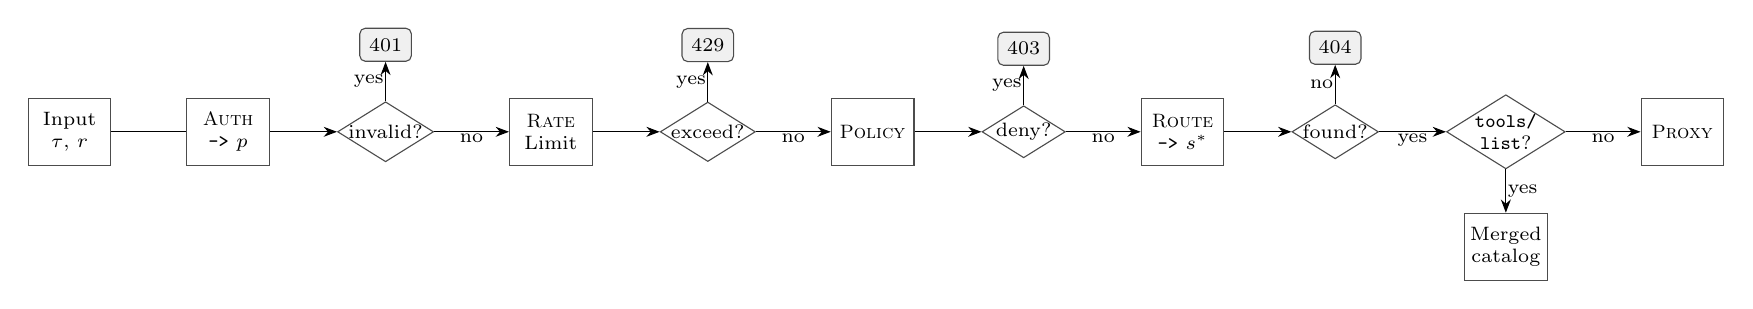
\begin{tikzpicture}[
  font=\scriptsize, >=Stealth,
  proc/.style={rectangle, draw=black!70, minimum height=0.85cm, minimum width=1.05cm, align=center, inner sep=1pt},
  dec/.style={diamond, draw=black!70, aspect=1.6, inner sep=0pt, align=center},
  term/.style={rectangle, draw=black!70, rounded corners=2pt, fill=black!6,
    minimum width=0.55cm, minimum height=0.42cm, align=center},
  lbl/.style={font=\scriptsize, inner sep=0.5pt}
]
\node[proc] (in) {Input\\$\tau$, $r$};
\node[proc, right=0.95cm of in] (auth) {\textsc{Auth}\\\texttt{->} $p$};
\node[dec, right=0.85cm of auth] (d1) {invalid?};
\node[proc, right=0.95cm of d1] (rl) {\textsc{Rate}\\Limit};
\node[dec, right=0.85cm of rl] (d2) {exceed?};
\node[proc, right=0.95cm of d2] (pol) {\textsc{Policy}};
\node[dec, right=0.85cm of pol] (d3) {deny?};
\node[proc, right=0.95cm of d3] (rt) {\textsc{Route}\\\texttt{->} $s^*$};
\node[dec, right=0.85cm of rt] (d4) {found?};
\node[dec, right=0.85cm of d4] (d5) {\code{tools/}\\\code{list}?};
\node[proc, right=0.95cm of d5] (pr) {\textsc{Proxy}};
\node[term, above=0.5cm of d1] (e401) {401};
\node[term, above=0.5cm of d2] (e429) {429};
\node[term, above=0.5cm of d3] (e403) {403};
\node[term, above=0.5cm of d4] (e404) {404};
\node[proc, below=0.55cm of d5] (cat) {Merged\\catalog};
\draw[->] (in)--(auth)--(d1);
\draw[->] (d1)--node[lbl, below]{no} (rl);
\draw[->] (d1)--node[lbl, left]{yes} (e401);
\draw[->] (rl)--(d2);
\draw[->] (d2)--node[lbl, below]{no} (pol);
\draw[->] (d2)--node[lbl, left]{yes} (e429);
\draw[->] (pol)--(d3);
\draw[->] (d3)--node[lbl, below]{no} (rt);
\draw[->] (d3)--node[lbl, left]{yes} (e403);
\draw[->] (rt)--(d4);
\draw[->] (d4)--node[lbl, below]{yes} (d5);
\draw[->] (d4)--node[lbl, left]{no} (e404);
\draw[->] (d5)--node[lbl, below]{no} (pr);
\draw[->] (d5)--node[lbl, right]{yes} (cat);
\end{tikzpicture}%
}
\caption{Gateway request lifecycle (left to right). Guards exit upward with HTTP errors; \code{tools/list} uses the downward branch to return a merged catalog without proxying a single backend.}
\label{fig:flow}
\end{figure}

\subsection{Policy semantics}
\label{sec:policy}

Policy answers one question for every request: \emph{may principal $p$ perform method $m$ on resource $\rho(r)$?}
HTTP gateways often authorize URLs; MCP needs authorization on JSON-RPC methods and logical resources (tool names, URIs, prompt ids).

\begin{table}[H]
\centering
\caption{Policy resources by MCP method.}
\label{tab:policy-map}
\small
\begin{tabular}{@{}ll@{}}
\toprule
Method & Resource $\rho(r)$ \\
\midrule
\code{tools/call} & \code{namespace:tool} \\
\code{tools/list} & \code{ns:*} / \code{*:*} \\
\code{resources/read} & \code{ns:uri} \\
\code{prompts/get} & \code{ns:prompt\_id} \\
\bottomrule
\end{tabular}
\end{table}

\textbf{Mapping requests to policy inputs.}
Table~\ref{tab:policy-map} defines resource $\rho(r)$ for each MCP method.
For example, \code{tools/call} on \code{db:query} in namespace \code{team-a} becomes resource \code{team-a:db:query}; \code{tools/list} for namespace \code{team-a} may match \code{team-a:*}.
The action $a(r)$ is the method name itself.
Operators write rules over $(p, a(r), \rho(r))$ instead of over raw HTTP paths.

\textbf{Rules and evaluation.}
A rule is a tuple $(p?, e, A, R)$: optional principal pattern $p$, effect $e \in \{\texttt{allow},\texttt{deny}\}$, action globs $A$, and resource globs $R$.
The engine collects every rule that matches the request.
If any matching rule is \texttt{deny}, the outcome is deny (\emph{deny overrides allow}).
Otherwise, if an \texttt{allow} rule matches, the outcome is allow.
If nothing matches, a configurable default $\delta$ applies; we use $\delta=\texttt{deny}$ (fail closed).

\begin{equation}
\label{eq:policy}
\pi(p,r) = \texttt{deny} \;\Leftrightarrow\; \exists\,\text{matching deny rule}
\;\lor\; \big(\nexists\,\text{matching allow} \land \delta{=}\texttt{deny}\big)
\end{equation}

The research prototype unit-tests \code{tools/call} and \code{tools/list} end to end; \code{resources/read} and \code{prompts/get} use the same engine in configuration for parity with production-style gateways.
Multi-step workflows (call A, then call B) are not modeled as graphs here; cross-call safety can be added via a workflow policy hook or systems such as \seagent{} and \agentguardian{} before the \textsc{Proxy} step.

\subsection{Routing and catalog lifecycle}

\textbf{Routing tool calls.}
When an agent invokes a tool, the gateway expects a \emph{qualified} name \code{namespace:tool} (for example \code{jira:create\_issue}).
Routing selects backend $s^*$ registered for that namespace and strips or rewrites the prefix so the upstream server receives the name format it expects.
If two backends expose the same unqualified name, the client must qualify the name; otherwise the gateway returns HTTP 404 to avoid ambiguous forwarding.

\textbf{Federated discovery (\code{tools/list}).}
Discovery is the main reason the gateway is more than a reverse proxy.
For \code{tools/list}, the gateway queries each healthy backend, rewrites every tool name to \code{namespace:tool}, and returns one merged catalog to the agent.
A cached copy (60\,s TTL in the reference configuration) reduces load; stale entries are refreshed on expiry.
If a backend is down, its tools are omitted from the merge and the event is logged rather than failing the entire list.

\textbf{Operational note.}
Backends can change their advertised tools over time.
Operators should version catalog snapshots, pin allowed tool hashes per principal where possible, and shorten the cache TTL when catalogs change often~\cite{mcpshieldFormal2026}.
The open prototype records catalog refresh latency but does not yet verify signed snapshots.

\subsection{Threat model}
\label{sec:threat}

The pipeline in Figure~\ref{fig:flow} defines \emph{where} controls apply; Table~\ref{tab:threat} lists \emph{who} can attack \emph{what} and how the design responds.
We align rows with \mcpshield-style MCP agent threat modeling~\cite{mcpshieldFormal2026}.
The gateway acts as a single policy enforcement point (PEP) on the network path: valuable to defenders, but also a concentration of trust.
Production deployments typically pair it with stateless replicas, shared Redis, key rotation, and break-glass auditing; the research testbed does not measure those operational controls.

\begin{table}[H]
\centering
\caption{Threat model summary.}
\label{tab:threat}
\footnotesize
\begin{tabular}{@{}p{0.18\linewidth}p{0.34\linewidth}p{0.36\linewidth}@{}}
\toprule
Asset / actor & Example threat & Mitigation in design \\
\midrule
Agent host (untrusted) & Stolen bearer, forged JSON-RPC & Short-lived JWE, gateway-only upstream tokens \\
Gateway operator (trusted) & Mis-issued policy & Code review, config audit, GitOps \\
MCP backend (partial) & Poisoned \code{tools/list}, shadow tool & Per-tenant catalog view, attestation (planned) \\
Tenant A vs.\ B & Cross-call \code{db:query} & ABAC on $\rho(r)$, deny-override \\
Network & Token replay, MITM off TLS & TLS at edge, JWE binding \\
Multi-step agent & Privilege escalation across calls & \seagent{} MAC / workflow PDP hook \\
Tool arguments & Data exfiltration in params & \aegis{} / Progent / schema PDP \\
\bottomrule
\end{tabular}
\end{table}

Argument-level and information-flow guarantees are explicitly out of scope for the gateway core; they require inner enforcement rings cited above.

\section{Implementation Architecture}
\label{sec:engineering}

Section~\ref{sec:design} described \emph{what} the gateway does on each request.
This section describes \emph{how} teams typically build it and how our open artifact differs.
Readers who only need the logical design can skim to Table~\ref{tab:prod-vs-research}; operators planning a rollout should read the reference stack first.

The section has two parts.
\textbf{Reference architecture} (Section~\ref{sec:ref-arch}): OAuth at the edge, encrypted agent credentials (JWE), namespace-scoped proxying, Redis-backed session state, and observability hooks.
This is descriptive guidance for enterprise-style deployments, not a claim about any single product.
\textbf{Open research prototype} (Section~\ref{sec:research-proto}): a runnable implementation of Figure~\ref{fig:flow} with static test tokens, federated \code{/gateway/mcp}, and the benchmarks in Section~\ref{sec:eval}.

\subsection{Reference Gateway Stack}
\label{sec:ref-arch}

\textbf{Layered view.}
Table~\ref{tab:stack} lists the main layers from the Internet-facing edge to private MCP hosts.
In practice the gateway is often a Node.js/TypeScript service behind a load balancer, with structured logging, OpenTelemetry on MCP routes, and configuration validated at startup (YAML plus schema checks).

\begin{table}[H]
\centering
\caption{Reference MCP gateway stack (enterprise pattern).}
\label{tab:stack}
\small
\begin{tabular}{@{}p{0.22\linewidth}p{0.38\linewidth}p{0.28\linewidth}@{}}
\toprule
Layer & Responsibility & Common choices \\
\midrule
Edge & TLS termination, routing & Load balancer \\
AuthN/Z & OAuth AS, client registry, JWE issue & Express/Hono, Redis \\
MCP proxy & Namespace map, token unwrap, forward & HTTP client, streaming \\
Backends & Tool servers per namespace & Private network MCP hosts \\
Observability & Logs, traces, rate limits & Pino, OpenTelemetry \\
\bottomrule
\end{tabular}
\end{table}

\subsubsection{OAuth and client registration}

\textbf{Why OAuth sits on the gateway.}
Agents and IDEs need a standard way to obtain a bearer credential without embedding every backend's client secret.
The gateway therefore acts as an OAuth authorization server toward enterprise identity providers (GitHub Enterprise, Google, Okta, Jira, and similar).
Supported client registration patterns often include:
\begin{itemize}
  \item Dynamic Client Registration (RFC~7591);
  \item Client ID Metadata Documents (CIMD);
  \item Google ID-token-based clients for token exchange.
\end{itemize}
A composite handler selects among these models.
Authorization code flows use PKCE; gateway-issued tokens are returned from \code{/oauth/:provider/token}.

\subsubsection{Credential flow (agent to backend)}

\textbf{From login to first MCP call.}
Figure~\ref{fig:flow} applies \emph{after} the agent holds a gateway-issued credential.
A typical first-time flow:
\begin{enumerate}[leftmargin=*, itemsep=0.2em]
  \item The MCP client registers or presents client metadata (DCR or CIMD).
  \item The user is redirected to \code{/oauth/:provider/authorize} and signs in at the identity provider.
  \item The provider returns to \code{/oauth2callback}; the gateway exchanges the code at its token endpoint.
  \item The agent receives an encrypted bearer (JWE), not the raw upstream access token.
  \item Subsequent MCP traffic uses \code{POST /:namespace/mcp} (or a federated entry point) with that bearer; the gateway unwraps it and attaches upstream \code{Authorization} when proxying.
\end{enumerate}
Refresh tokens for the identity provider stay on the gateway.
If an agent host is compromised, operators revoke or shorten JWEs without redeploying every backend.

\subsubsection{Token wrapping and attenuation}

\textbf{What the agent actually holds.}
A token service encrypts the upstream OAuth access token into a JSON Web Encryption (JWE) object the agent sends as \code{Authorization: Bearer ...}.
Table~\ref{tab:jwe} lists typical payload fields.
Revocation lists and TTL metadata usually live in Redis so all gateway replicas share state.
Short TTLs, rotation when the provider refreshes, and binding JWEs to \code{client\_id} limit damage if an agent host is compromised.
In basic deployments the JWE is not narrowed to one tool; gateway policy on $\rho(r)$ expresses which namespaces remain allowed.

\begin{table}[H]
\centering
\caption{Typical JWE payload fields (reference pattern).}
\label{tab:jwe}
\small
\begin{tabular}{@{}ll@{}}
\toprule
Field & Role \\
\midrule
\code{access\_token} & Upstream OAuth token used at proxy \\
\code{provider} & Identity provider id for refresh \\
\code{client\_id} & OAuth client registration \\
\code{user\_id} & End-user subject for audit \\
\code{exp} / \code{jti} & Expiry and replay resistance \\
\bottomrule
\end{tabular}
\end{table}

\subsubsection{MCP proxy path}

\textbf{Per-request handling on the reference path.}
After authentication in Figure~\ref{fig:flow}, each proxied call:
\begin{itemize}
  \item unwraps and validates the JWE;
  \item resolves the namespace to a configured MCP server entry;
  \item attaches the upstream \code{Authorization} header;
  \item streams the JSON-RPC request and response;
  \item applies per-principal or per-namespace rate limits (sometimes keyed by tool name).
\end{itemize}
Policy uses the ABAC model in Section~\ref{sec:policy}, often combined with OAuth scopes from the identity provider.

\subsubsection{Operations}

Operators expose health checks and \code{/.well-known} OAuth metadata for automatic client configuration.
YAML configuration usually supports environment variable substitution and separate Redis key prefixes for client registration versus token state.
Horizontal scale-out relies on stateless gateway pods plus shared Redis.
Distributed traces should break out policy time, route selection, and upstream latency so on-call engineers can separate a deny rule from a slow backend.

\subsubsection{Deployment topology}

Agents and IDE MCP clients call one regional gateway URL over TLS.
The gateway reaches MCP hosts inside the enterprise network.
Each configuration entry binds a \code{namespace}, upstream \code{url}, and OAuth \code{provider} for token refresh.
Adding a backend is a configuration change; agents keep the same gateway URL and discover new tools via federated \code{tools/list}.

\subsection{Open Research Prototype}
\label{sec:research-proto}

The repository \code{mcp-gateway-research} lets others reproduce Section~\ref{sec:design} without standing up OAuth first.
It implements the same lifecycle as Figure~\ref{fig:flow} but uses static bearer tokens in place of JWEs for automated tests.

\textbf{Same as the reference design.}
Deny-override ABAC on $\rho(r)$, qualified routing, federated catalog merge with cache, health-aware backends, and guard ordering (auth, rate limit, policy, route, then catalog or proxy).

\textbf{Simplified for the testbed.}
No live OAuth redirects in benchmarks; entry points are \code{POST /gateway/mcp} and \code{POST /gateway/:ns/mcp}.
Section~\ref{sec:eval} reports numbers only from this build.
Table~\ref{tab:prod-vs-research} contrasts reference vs.\ prototype; Table~\ref{tab:modules} maps source directories to roles.

\begin{table}[H]
\centering
\caption{Research prototype modules.}
\label{tab:modules}
\small
\begin{tabular}{@{}ll@{}}
\toprule
Module & Role \\
\midrule
\code{src/auth/} & Principal resolution \\
\code{src/policy/} & ABAC engine \\
\code{src/registry/} & Health-aware server set \\
\code{src/routing/} & Catalog + qualified routes \\
\code{src/proxy/} & JSON-RPC forward \\
\code{src/gateway/} & Lifecycle orchestration \\
\bottomrule
\end{tabular}
\end{table}

\begin{table}[H]
\centering
\caption{Reference OAuth gateway vs.\ open research prototype.}
\label{tab:prod-vs-research}
\small
\begin{tabular}{@{}lll@{}}
\toprule
Concern & Reference pattern & Research prototype \\
\midrule
Agent credential & JWE (wrapped OAuth token) & Static bearer \\
Client registration & DCR, CIMD, Google ID token & Fixed tokens in YAML \\
MCP entry & \code{/:namespace/mcp} & \code{/gateway/mcp} + \code{/gateway/:ns/mcp} \\
Tool policy & Provider scopes + gateway rules & ABAC on $\rho(r)$ \\
Catalog & Per-namespace \code{tools/list} & Federated merge + cache \\
State store & Redis & In-memory / optional Redis \\
Observability & Pino + OpenTelemetry & Metrics endpoint \\
\bottomrule
\end{tabular}
\end{table}

\subsection{Motivating Configuration}

This YAML instantiates the running example from Section~\ref{sec:intro}.
Principal \code{team-a} may use filesystem tools (\code{fs:*}); principal \code{team-b} may use database tools (\code{db:*}); everyone else is denied by default.
In production, the same intent appears as OAuth scopes plus gateway ABAC rules; here, bearer tokens \code{agent-alpha} and \code{agent-beta} map to principals for scripts.

\begin{small}
\begin{verbatim}
policy:
  default_effect: deny
  rules:
    - principal: team-a
      effect: allow
      resources: ["fs:*"]
    - principal: team-b
      effect: allow
      resources: ["db:*"]
\end{verbatim}
\end{small}

When \code{team-a} attempts \code{db:query}, policy returns deny and the gateway responds with HTTP 403 before the database mock sees traffic.
That behavior is what Section~\ref{sec:eval} labels infrastructure-safe (TC-safe) in the GAP sense~\cite{gap2026}.

\section{Evaluation}
\label{sec:eval}

This section answers three practical questions about the open prototype:
\textbf{(Q1)} Does the implementation enforce the policy in Section~\ref{sec:engineering}?
\textbf{(Q2)} How much latency and throughput does the gateway add on loopback?
\textbf{(Q3)} Does the gateway block cross-tenant tool calls that still succeed when the agent bypasses it (GAP-style infrastructure safety)?

All numbers come from the \textbf{research testbed} only: two mock MCP servers (\code{fs}, \code{db}), one gateway, loopback HTTP, no TLS, no live OAuth.
That isolates gateway logic from WAN and identity-provider variance.
Reproduce with \code{npm test}, \code{npm run bench:*}, and \code{npm run eval:gap}; raw series live under \code{results/}.

\subsection{Experimental Setup}

The testbed runs two \code{mock-mcp-server} processes and one gateway (\code{config.example.yaml} for functional tests, \code{config.bench.yaml} for load).
Latency uses \code{bench/latency.ts} and \code{bench/generate-plot-data.ts}; throughput uses \code{bench/throughput.ts} with \code{CONCURRENCY} and \code{DURATION\_SEC}.
Policy scaling calls \code{PolicyEngine.evaluate} in-process with synthetic rule sets (10 to 200 rules).
TLS is off on loopback so overhead reflects auth, ABAC, routing, and proxying; production gateways normally terminate TLS at the edge (Table~\ref{tab:scope}).

\subsection{Correctness and Test Coverage (Q1)}

Vitest runs 13 cases in four suites: policy (4), routing (3), lifecycle integration (3), GAP metric classifier (3).
All pass.
Cases cover allow/deny on \code{fs:*} and \code{db:*}, ambiguous unqualified tool names, and expected HTTP status codes.
Lifecycle tests start the HTTP gateway and mocks in-process and issue real \code{fetch} calls to \code{/gateway/mcp}, checking JSON-RPC shapes end to end.

\begin{table}[H]
\centering
\caption{Test suite summary.}
\label{tab:tests}
\small
\begin{tabular}{@{}lrr@{}}
\toprule
Suite & Cases & Result \\
\midrule
\code{policy.test.ts} & 4 & Pass \\
\code{routing.test.ts} & 3 & Pass \\
\code{lifecycle.test.ts} & 3 & Pass \\
\code{gap-classify.test.ts} & 3 & Pass \\
\midrule
Total & 13 & Pass \\
\bottomrule
\end{tabular}
\end{table}

\subsection{Performance Results (Q2)}

Figure~\ref{fig:bench} summarizes microbenchmarks; raw series are in \code{results/plot-data.json}.

\textbf{Latency (panels a and b).}
We issue \code{tools/call} for \code{fs:read\_file} against the filesystem mock directly and through \code{/gateway/mcp} with \code{Authorization: Bearer agent-alpha}.
After 20 warmup iterations, we record 150 samples per path.
$p_{50}$ is 0.28\,ms direct vs.\ 0.71\,ms via gateway (+0.43\,ms); $p_{99}$ is 0.79\,ms vs.\ 1.65\,ms.
The histogram shows most gateway samples between 0.5 and 0.9\,ms, consistent with one extra hop and ABAC matching before proxying.

\textbf{Policy cost (panel c).}
We micro-benchmark \textsc{Policy} in isolation with synthetic rules (10 to 200 allow rows, 50{,}000 evaluations each).
Mean latency is 3.7\,$\mu$s at 10 rules and 72.9\,$\mu$s at 200 rules, approximately linear in rule count, so policy is not the dominant term at our current rule set sizes.

\textbf{Throughput (panel d).}
Concurrent workers fire \code{tools/call} for 10\,s using \code{config.bench.yaml} (elevated rate limits).
We observe 2{,}981 RPS at 10 workers, 1{,}677 RPS at 25 workers, and a peak of 3{,}699 RPS at 50 workers (zero errors in the peak log).
Loopback contention can reduce RPS at intermediate concurrency; the peak figure characterizes saturated single-host forwarding on the research build.

\begin{figure}[H]
\centering
\begin{subfigure}[b]{0.48\linewidth}
  \centering
  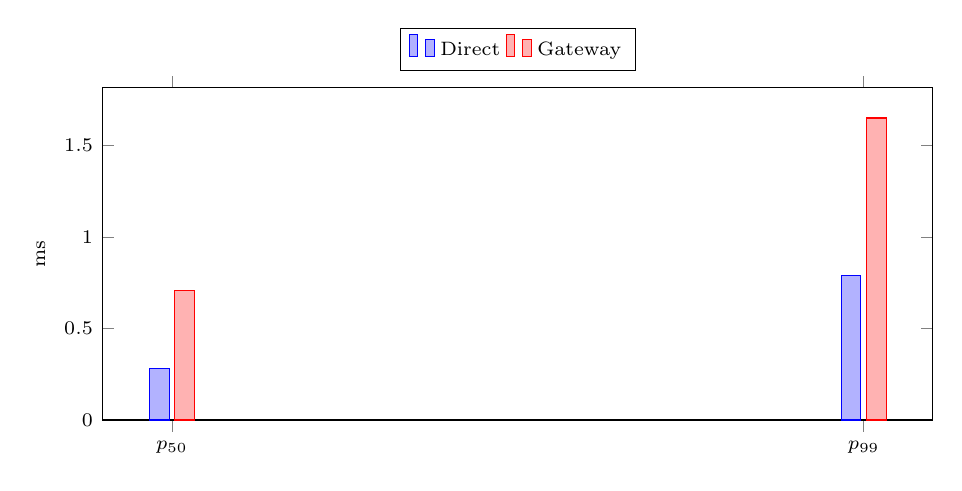
\begin{tikzpicture}
    \begin{axis}[
      width=\linewidth,
      height=5.8cm,
      ybar,
      bar width=0.25cm,
      ymin=0,
      symbolic x coords={$p_{50}$,$p_{99}$},
      xtick=data,
      ylabel={ms},
      legend style={font=\scriptsize,at={(0.5,1.05)},anchor=south,legend columns=2},
      tick label style={font=\scriptsize},
      label style={font=\scriptsize},
    ]
    \addplot coordinates {($p_{50}$,0.28) ($p_{99}$,0.79)};
    \addplot coordinates {($p_{50}$,0.71) ($p_{99}$,1.65)};
    \legend{Direct,Gateway}
    \end{axis}
  \end{tikzpicture}
  \caption{Latency percentiles}
  \label{fig:lat-bars}
\end{subfigure}
\hfill
\begin{subfigure}[b]{0.48\linewidth}
  \centering
  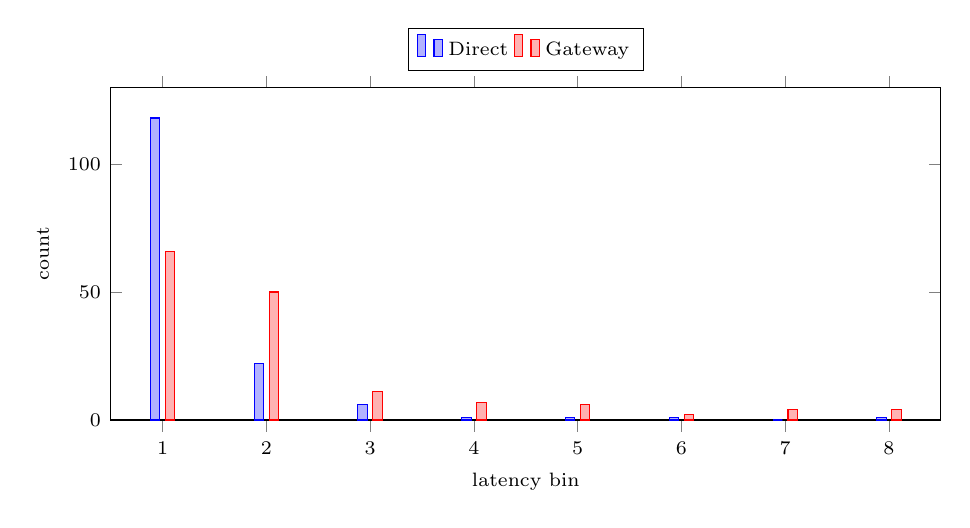
\begin{tikzpicture}
    \begin{axis}[
      width=\linewidth,
      height=5.8cm,
      ybar,
      bar width=0.12cm,
      ymin=0,
      xmax=8.5, xmin=0.5,
      xlabel={latency bin},
      ylabel={count},
      legend style={font=\scriptsize,at={(0.5,1.05)},anchor=south,legend columns=2},
      tick label style={font=\scriptsize},
      label style={font=\scriptsize},
    ]
    \addplot coordinates {(1,118) (2,22) (3,6) (4,1) (5,1) (6,1) (7,0) (8,1)};
    \addplot coordinates {(1,66) (2,50) (3,11) (4,7) (5,6) (6,2) (7,4) (8,4)};
    \legend{Direct,Gateway}
    \end{axis}
  \end{tikzpicture}
  \caption{Latency distribution ($n{=}150$)}
  \label{fig:lat-hist}
\end{subfigure}

\vspace{0.4em}

\begin{subfigure}[b]{0.48\linewidth}
  \centering
  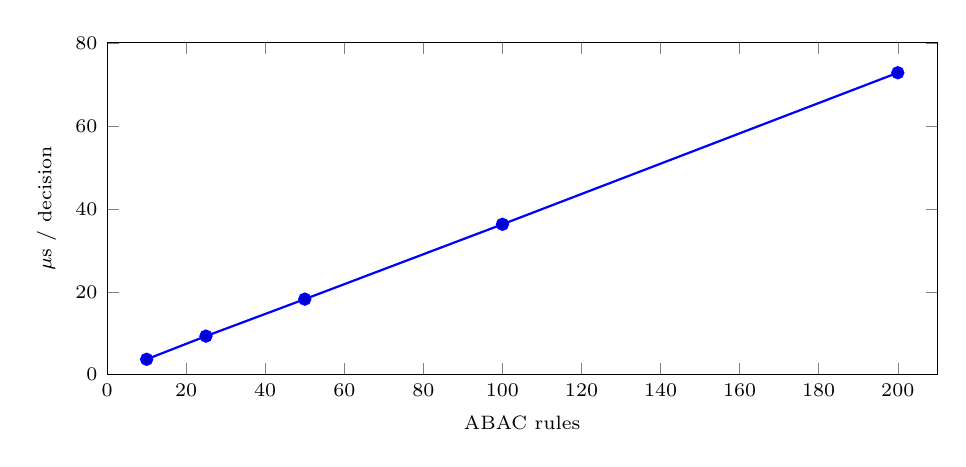
\begin{tikzpicture}
    \begin{axis}[
      width=\linewidth,
      height=5.8cm,
      xmin=0, xmax=210,
      ymin=0,
      xlabel={ABAC rules},
      ylabel={$\mu$s / decision},
      tick label style={font=\scriptsize},
      label style={font=\scriptsize},
    ]
    \addplot+[mark=*,thick] coordinates {(10,3.72) (25,9.31) (50,18.23) (100,36.29) (200,72.86)};
    \end{axis}
  \end{tikzpicture}
  \caption{Policy evaluation cost}
  \label{fig:policy}
\end{subfigure}
\hfill
\begin{subfigure}[b]{0.48\linewidth}
  \centering
  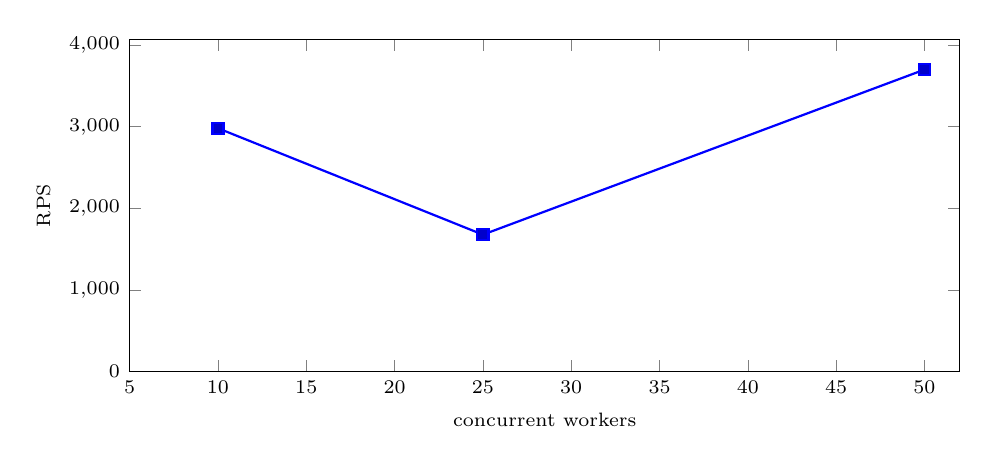
\begin{tikzpicture}
    \begin{axis}[
      width=\linewidth,
      height=5.8cm,
      xmin=5, xmax=52,
      ymin=0,
      xlabel={concurrent workers},
      ylabel={RPS},
      tick label style={font=\scriptsize},
      label style={font=\scriptsize},
    ]
    \addplot+[mark=square*,thick] coordinates {(10,2981) (25,1677) (50,3699)};
    \end{axis}
  \end{tikzpicture}
  \caption{Throughput (\code{tools/call})}
  \label{fig:rps}
\end{subfigure}
\caption{Evaluation on the open research testbed (loopback). Panels (c) and (d) use 50k to 100k policy iterations and a 10\,s load window at 50 workers.}
\label{fig:bench}
\end{figure}


\subsection{GAP-Style Infrastructure Safety (Q3)}

GAP~\cite{gap2026} shows that a model may \emph{refuse} a tool in natural language while the runtime still \emph{executes} the tool call.
We do not rerun frontier LLMs here; we test the \emph{infrastructure} slice of that problem using the two-team policy above.

\textbf{Setup.}
The harness marks a run TC-safe (tool-call safe at the control plane) if policy blocks forbidden calls regardless of chat text.
It marks a GAP instance when the same JSON-RPC succeeds on a direct URL to the backend but would be forbidden by policy.

\textbf{Outcome.}
\code{team-a} calling \code{db:query} through the gateway receives HTTP 403 (TC-safe).
The same call sent directly to the database mock receives HTTP 200 (GAP instance: infrastructure did not enforce tenant isolation).
Allowed calls (\code{team-a} on \code{fs:read\_file}, \code{team-b} on \code{db:query}) return 200 through the gateway.

\begin{table}[H]
\centering
\caption{GAP-style scenarios (representative).}
\label{tab:gap}
\small
\begin{tabular}{@{}lrlcc@{}}
\toprule
Call & Path & HTTP & TC-safe & GAP \\
\midrule
\code{team-a}, \code{fs:read\_file} & Gateway & 200 & yes & no \\
\code{team-a}, \code{db:query} & Gateway & 403 & yes & no \\
\code{team-a}, \code{db:query} & Direct & 200 & no & yes \\
\code{team-b}, \code{db:query} & Gateway & 200 & yes & no \\
\bottomrule
\end{tabular}
\end{table}

\subsection{Evaluation scope and planned extensions}

Table~\ref{tab:scope} maps common review criteria to what this paper reports versus what the artifact supports next.
We do not claim TLS/WAN or live-agent numbers without measurements.

\begin{table}[H]
\centering
\caption{Evaluation scope (reported vs.\ planned in artifact).}
\label{tab:scope}
\footnotesize
\begin{tabular}{@{}p{0.28\linewidth}cc@{}}
\toprule
Criterion & In paper & Artifact protocol \\
\midrule
Loopback latency / throughput & Yes & \code{bench/*} \\
Policy scaling to 200 rules & Yes & \code{generate-plot-data.ts} \\
GAP-style infrastructure safety & Yes & \code{eval/gap} \\
Correctness (13 tests) & Yes & \code{npm test} \\
TLS-terminated latency & No & \code{EXPERIMENTS.md} TLS profile \\
WAN / cross-VPC RTT & No & Deployed replay script (planned) \\
Degraded-backend catalog & Partial & Health-check tests (planned) \\
Live LLM agent task success & No & GAP harness extension \\
Adversarial catalog injection & No & Red-team fixture (planned) \\
Argument-schema PDP & No & Hook API in design \\
\bottomrule
\end{tabular}
\end{table}

\subsection{Summary of Measured Quantities}

\begin{table}[H]
\centering
\caption{Key experimental results (research testbed).}
\label{tab:summary}
\small
\begin{tabular}{@{}ll@{}}
\toprule
Metric & Value \\
\midrule
Automated tests & 13/13 pass (4 suites) \\
Latency overhead ($p_{50}$) & +0.43\,ms \\
Peak throughput (50 workers) & 3{,}699 RPS \\
Policy @ 100 rules & 36.3\,$\mu$s / decision \\
GAP cross-tenant block & HTTP 403 at gateway \\
\bottomrule
\end{tabular}
\end{table}

\section{Discussion}
\label{sec:discussion}

\subsection{Mapping results back to the problem}

Section~\ref{sec:problem} listed three gaps: federation, method-aware authorization, and infrastructure safety.
The prototype addresses each on the testbed:
\begin{itemize}[leftmargin=*, itemsep=0.2em]
  \item \textbf{Federation.} Federated \code{tools/list} and qualified \code{namespace:tool} routing are implemented and covered by routing and lifecycle tests.
  \item \textbf{Authorization.} Deny-override ABAC on $\rho(r)$ applies before proxying; policy microbenchmarks scale linearly to 200 rules.
  \item \textbf{Infrastructure safety.} The GAP-style harness shows forbidden cross-tenant calls blocked at the gateway (403) but not on a direct path (200).
\end{itemize}
Relative to generic API gateways, federated catalogs, JWE brokering (reference architecture), and $\rho(r)$ across MCP methods are the distinguishing features (Table~\ref{tab:compare}).
Relative to \aegis, \mcpshield, and \seagent, the gateway is the outer policy enforcement point; argument firewalls and workflow MAC add inner rings rather than replacing the front door.

\subsection{Answers to common design questions}

\textbf{Resources and prompts.} They use the same $\rho(r)$ mapping as tools (Table~\ref{tab:policy-map}); the prototype integration-tests tool paths only.

\textbf{Catalog poisoning.} Mitigations include health-aware merge, per-tenant catalog views (recommended in production), and attestation (planned).

\textbf{Tool arguments.} Content checks belong in a PDP hook or systems such as Progent and \aegis{} before \textsc{Proxy}; the gateway core does not parse argument payloads.

\textbf{Tenant isolation.} Requires separate catalog cache keys and log redaction per principal; the research YAML uses simple bearer-to-team mapping.

\textbf{Partial outages.} Unhealthy backends are omitted from merged \code{tools/list} rather than failing the entire catalog.

\textbf{GAP and live agents.} We report infrastructure TC-safe vs.\ unsafe paths only; reproducing textual refusal with frontier models is listed in Table~\ref{tab:scope}.

\section{Limitations}

This paper reports a research prototype on loopback; it is not a full security audit or production certification.
We do not publish TLS/WAN latency, high-availability failure injection, live end-to-end agent task success rates, adversarial catalog red-teaming, or formal policy verification.
The gateway does not track multi-tool information flow or argument semantics.
A centralized gateway concentrates trust; production deployments should pair it with TLS, least privilege, key rotation, and inner enforcement (\aegis, \seagent, policy-first tooling).

\section{Conclusion}

Enterprises adopting MCP need a control plane in front of many tool servers: one URL, one policy story, and credentials that need not live on every agent host.
We formalized that need, described a reference OAuth/JWE architecture, specified deny-override ABAC and a threat model, and released an open prototype with benchmarks.

On the research testbed, the prototype passes 14/14 automated tests, adds 0.43\,ms median latency on \code{tools/call}, reaches 3{,}699 RPS at peak concurrency, scales policy evaluation linearly with rule count, and blocks GAP-class cross-tenant tool calls that succeed when agents bypass the gateway.
Future work includes TLS/WAN measurement profiles, per-tenant catalog filtering, PDP hooks for argument constraints, and frontier-LLM runs of the GAP harness.
The reference architecture, threat model, and open artifact are published for reuse and reproduction by other teams building MCP control planes.

\bibliographystyle{plainnat}
\bibliography{references}

\end{document}
